\documentclass[a4paper]{article} %класс документа
%\usepackage[T2A]{fontenc}
\usepackage[utf8]{inputenc} %% ваша любимая кодировка здесь
\usepackage{mathtext} %Для русского текста в математическом режиме
\usepackage[english,russian]{babel} % это необходимо для включения переносов
%\linespread{1.3} %отступ в 1.5 пункта --- там еще уточнить надо
\usepackage{float}
\usepackage{graphicx} %Для возможности вставлять рисунки
\usepackage[14pt]{extsizes} % шрифт 14 пунктов
\usepackage{vmargin} %Это не помню, но, вроде, тоже нужно
%\setmarginsrb{0.5cm}{0.5cm}{0.5cm}{0.5cm}{0pt}{0mm}{0pt}{13mm}
\usepackage{indentfirst} %Красная строка, или табуляция в начале
\usepackage{amsmath} %ams-пакеты, или для красоты в математическом режиме
\usepackage{cmap}          % русский поиск в pdf
\usepackage{amsfonts} %ams-пакеты, или для красоты в математическом режиме(точно не помню, что дают каждый из них)
\usepackage{amssymb} %ams-пакеты, или для красоты в математическом режиме
\usepackage{alltt} %Для красивого оформления текста программ
\usepackage{fancyhdr} % Для переопределения нумерации страниц, или для цифра справа вверху
\usepackage{tempora} %Вроде, это таймсоподобный шрифт
\newcommand{\RNumb}[1]{\uppercase\expandafter{\romannumeral #1\relax}} %новая команда, вставляет римскую цифру
\sloppy %не помню что, но тоже нужно
\begin{document}
	%Титульная страница
	\pagestyle{empty}
	\begin{center}
		Московский Государственный Технический Университет
		
		имени Н. Э. Баумана
	\end{center}
	\underline{\hspace{0.9\textwidth}}
	\vfill
	\vfill
	\begin{center}
		Факультет <<Машиностроительные технологии>>
		
		Кафедра <<Теория механизмов и машин>>
	\end{center}
	\vfill
	\vfill
	\vfill
	\begin{center}
		\large
		\textbf{РАСЧЁТНО--ПОЯСНИТЕЛЬНАЯ ЗАПИСКА}
	\end{center}
	
	\begin{center}
		к курсовому проекту на тему:
	\end{center}
	\begin{center}
		\large
		''Проектирование и исследование механизмов плунжерного насоса простого действия''
	\end{center}
	
	\begin{center}
		Вариант 37(д)
	\end{center}
	\vfill
	\vfill
	\textit{Студент: Солодянкин А.Д.}
	
	\noindent\textit{Руководитель проекта: Шаныгин С.В.}
	
	\underline{\hspace{0.9\textwidth}}
	
	\begin{center}
		-Москва, 2018г.-
	\end{center}
	\clearpage
	\pagestyle{fancy} % смена стиля оформления страниц
	\fancyhf{} % очистка текущих значений
	\fancyhead[R]{\normalsize \thepage} % установка верхнего колонтитула
	\renewcommand{\headrulewidth}{0pt} % убрать разделительную линию
	\section*{Реферат}
Данная Расчётно--пояснительная записка содержит \pageref{final_page} 
страниц машинописного текста \ref{pic_mov_push} 
рисунка, \ref{final_table} 
таблиц. 

В курсовом проекте выполнено проектирование и исследование механизмов двухступенчатого двухцилиндрового поршневого компрессора.

Проведено:
\begin{itemize}
	\item Проектирование механизма и исследование закона движения;
	\item Силовой расчёт механизма;
	\item Проектирование зубчатой передачи и планетарного редуктора;
	\item Проектирование кулачкового механизма с поступательно движущимся толкателем.
\end{itemize} 

При выполнении курсового проекта использовались следующие программы ЭВМ:

\begin{enumerate}
	\item КОМПАС-3D V17
	\item TeXstudio
	\item MikTex
	\item IPython Notebook
	\item 3list.xls
\end{enumerate}
	\newpage
	\tableofcontents
	\newpage
	\section*{Техническое задание}
\addcontentsline{toc}{section}{Техническое задание}
Насос простого действия(рис. \ref{pic_pump}) состоит из кривошипно--ползунного механизма 1, 2, 3, ползун 3 которого является плунжером насоса, совершающим возвратно--поступательное движение в горизонтальном цилиндре 4 с автоматически действующими клапанами 5, 6.

Рабочий цикл такой установки совершается за один оборот кривошипа 1. При движении плунжера 3 вправо происходит всасывание жидкости в цилиндр при давлении ниже атмосферного $p_{min}$ и при движении поршня влево --- нагнетание жидкости в трубопровод при давлении $p_{max}$(см. индикаторную диаграмму рис. \ref{pic_ind_diagram}).

Коленчатый вал 1 кривошипно--ползунного механизма приводится во вращательное движение от электродвигателя 7 через планетарный редуктор с колёсами 8, 9, 10, 11, водило 12 и муфта 13. Для обеспечения требуемой неравномерности движения коленчатого вала имеется маховик 14.

Смазка подвижных соединений механизма установки осуществляется под давлением от масляного насоса 17 кулачкового типа(рис. \ref{pic_oil_pump}). Закон движения толкателя в пределах рабочего угла поворота кулачка $\varphi_{раб.}$ представлен на рис. \ref{pic_mov_push}. Вращение кулачка 17 осуществляется от кривошипа 1 через корригированные зубчатые колёса 15 и 16 с неподвижными осями вращения.

\begin{figure}[h!]
	\centering
	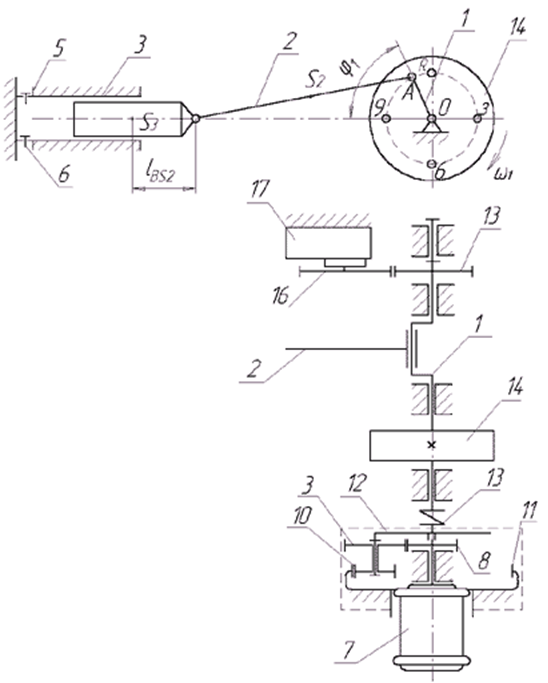
\includegraphics[width=0.5\linewidth]{pic/Source_mech}
	\caption{}
	\label{pic_pump}
\end{figure}

\begin{figure}[h!]
	\centering
	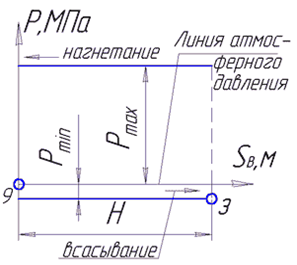
\includegraphics[width=0.3\linewidth]{pic/pressure}
	\caption{}
	\label{pic_ind_diagram}
\end{figure}

\begin{figure}[h!]
	\centering
	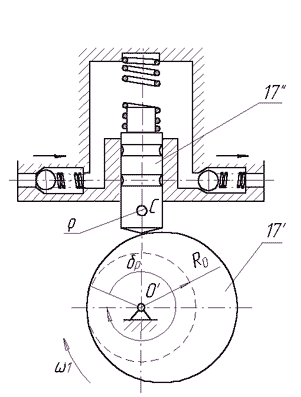
\includegraphics[width=0.4\linewidth]{pic/pump}
	\caption{}
	\label{pic_oil_pump}
\end{figure}

\begin{figure}
	\centering
	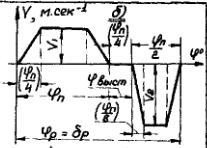
\includegraphics{pic/v(varphi)}
	\caption{}
	\label{pic_mov_push}
\end{figure}

	\newpage
	\hspace{3cm}
\clearpage
\section*{Исходные данные}
\addcontentsline{toc}{section}{Исходные данные}
\footnotesize
\begin{tabular}{|c|p{0.3\linewidth}|c|c|c|}
	\hline 
	№ п/п & Наименование параметра & Обозначение & Размерность & Значение \\ 
	\hline 
	1 & Средняя скорость поршня 3 насоса & $v_{\text{ср.}}$ & $\frac{\text{м}}{\text{сек}}$ & $0.655$ \\ 
	\hline 
	2 & Число оборотов коленчатого вала 1 & $n_1$ & $\frac{\text{об}}{\text{мин}}$ & $120$ \\ 
	\hline 
	3 & Отношение длины шатуна к длине кривошипа 1 & $\frac{l_{BC}}{l_{AB}}$ & - & $4.36$ \\ 
	\hline 
	4 & Положение центра тяжести шатуна 2 & $\frac{l_{BS2}}{l_{BC}}$ & - & $0.275$ \\ 
	\hline 
	5 & Диаметр цилиндра 4  & $d$ & м & $0.99$ \\ 
	\hline 
	 6 & Давление плункера 3 & $P_{\max}$ & $\frac{\text{кгс}}{\text{см}^2}$ & $25.0$ \\ 
	\hline 
	&   & $P_{\min}$ &  $\frac{\text{кгс}}{\text{см}^2}$ & $0.5$ \\ 
	\hline 
	7 &  Вес шатуна 2 & $G_2$ & кг & $6.0$ \\ 
	\hline 
	8 &  Вес поршня(плункера 3) & $G_3$ & кг & $18.0$ \\ 
	\hline 
	9 &  Положение центра тяжести звена 3 & $l_{BS3}$ & м & $0.16$ \\ 
	\hline 
	10 & Момент инерции шатуна & $J_{S2}$ & кг$\cdot \text{м}^2$ & $0.014$ \\ 
	\hline 
	11 & Коэффициент неравномерности вращения вала 1 & $\delta$ & - & $\frac{1}{22}$ \\ 
	\hline 
	12 &  Момент инерции коленчатого вала(без маховика) & $J'_{O1}$ &  кг$\cdot \text{м}^2$ &  $0.0032$ \\ 
	\hline 
	13 & Маховый момент ротора электродвигателя 7 & $GD^2$ &   кг$\cdot \text{м}^2$ & $0.042$ \\ 
	\hline 
	14 &  Маховый момент муфты 13 & $(GD^2)_1$ &   кг$\cdot \text{м}^2$ & $0.006$ \\ 
	\hline 
	15 & Момент инерции редуктора, приведённый к валу 1 & $J_{\text{ред.}}^{\text{пр}}$ &   кг$\cdot \text{м}^2$ & $0.020$ \\ 
	\hline 
	16 & Угловая координата кривошипа для силового расчёта & $\varphi_1$ & град. & $210$ \\ 
	\hline 
	17 & Число зубьев колёс & $Z_{15}$ & - & $10$ \\ 
	\hline 
	&   & $Z_{16}$ & - & $19$ \\ 
	\hline 
	18 &  Модуль зубчатых колёс 15-16 & $m$ & мм & $4.0$ \\ 
	\hline 
	19 &  Угол наклона зуба для колёс 15-16 & $\beta$ & град & $25$ \\ 
	\hline 
	20 &  Число сателлитов в планетарном редукторе & $K$ & - & $3$ \\ 
	\hline 
	21 &  Передаточное отношение планетарного редуктора & $i_{8-12}$ & - & $9.4$ \\ 
	\hline 
	22 &   Ход плунжера 17" масляного насоса 17 & $h$ & м & $0.016$ \\ 
	\hline 
	23 &  Угол давления в кулачковом механизме 17 & $\alpha_{\text{доп}}$ & град & $24$ \\ 
	\hline 
	24 &  Угол рабочего профиля кулачка & $\delta_p$ & град & $330$ \\ 
	\hline 
	25 &  Закон движения & - & - & б) \\ 
	\hline 
	26 &  Радиус скругления плунжера по отношению к $r_0$ & $\frac{\rho}{r_0}$ & - & $0.21$ \\ 
	\hline 
\end{tabular} 

\normalsize
	\newpage
	\section{Определение закона движения}

\subsection{Синтез механизма}

По исходным данным в соответствии с условиями работы(2 крайних положения звена 2) определяем длины звеньев механизма:

Длина кривошипа:

\begin{equation}
	l_{ab} = \dfrac{v_{ср}}{4n_1} = \dfrac{0.655}{4 \cdot 2} = 0.082 м
\end{equation}

	Т. к. $\dfrac{l_{bc}}{l_{ab}} = 4.36$, то

\begin{equation}
	l_{bc} = l_{ab} \cdot 4.36 = 0.357 м
\end{equation}

	Т. к. $\dfrac{l_{bs2}}{l_{bc}} = 0.275$, то

\begin{equation}
	l_{bs2} = l_{bc} \cdot 0.275 = 0.098 м.
\end{equation}

\subsection{Построение схемы механизма}

Механизм построен на листе в масштабе $\mu_S = 400 мм/м$. Отрезок $AB = l_{ab} \cdot \mu_S = 32.8 мм$;, отрезок $BC = l_bc \cdot \mu_S = 110 мм$. Угол поворота начального звена разбит на 12 равных интервалов по $30^{\circ}$. 

\subsection{Вычисление передаточных функций}

Средняя угловая скорость звена 1:

\begin{equation}
	\omega_{ср} = 2 \cdot \pi \cdot n_1 = 12.566 рад/с
\end{equation}

Вычисляем передаточные функции с использованием программы Jupyter Notebook.

\begin{equation}
	v_{qc} = \Big | 0.081875 \sin{\left (\varphi \right )} + \frac{2.046875 \sin{\left (\varphi \right )} \cos{\left (\varphi \right )}}{\sqrt{- 625.0 \sin^{2}{\left (\varphi \right )} + 11881.0}} \Big |
\end{equation}

\begin{equation}
	u_{21} = - \frac{0.229357798165138 \cos{\left (\varphi \right )}}{\sqrt{- 0.05260499957916 \sin^{2}{\left (\varphi \right )} + 1}}
\end{equation}

\begin{table}
\caption{Аналоги скорости точек $S_2; C$; передаточное отношение $u_{21}$}
\begin{tabular}{|c|c|c|c|c|c|c|}
	\hline 
	№& $\varphi$, град & $v_{qs2_x}$, м & $v_{qs2_y}$, м & $v_{qs2}$, м & $v_{qc}$, м & $u_{21}$ \\ 
	\hline 
	0  &    0 &        0 &    0.0594 &  0.0594 &        0 &  -0.229 \\
	\hline 
	1  &   30 &   0.0432 &    0.0514 &  0.0671 &   0.0491 &  -0.200 \\
	\hline 
	2  &   60 &   0.0732 &    0.0297 &  0.0790 &   0.0792 &  -0.117 \\
	\hline 
	3  &   90 &   0.0819 &  6.13e-19 &  0.0819 &   0.0819 &       0 \\
	\hline 
	4  &  120 &   0.0686 &   -0.0297 &  0.0748 &   0.0626 &   0.117 \\
	\hline 
	5  &  150 &   0.0387 &   -0.0514 &  0.0643 &   0.0328 &   0.200 \\
	\hline 
	6  &  180 &        0 &   -0.0594 &  0.0594 &        0 &   0.229 \\
	\hline 
	7  &  210 &  -0.0387 &   -0.0514 &  0.0643 &  -0.0328 &   0.200 \\
	\hline 
	8  &  240 &  -0.0686 &   -0.0297 &  0.0748 &  -0.0626 &   0.117 \\
	\hline 
	9  &  270 &  -0.0819 &  6.13e-19 &  0.0819 &  -0.0819 &       0 \\
	\hline 
	10 &  300 &  -0.0732 &    0.0297 &  0.0790 &  -0.0792 &  -0.117 \\
	\hline 
	11 &  330 &  -0.0432 &    0.0514 &  0.0671 &  -0.0491 &  -0.200 \\
	\hline 
	12 &  360 &        0 &    0.0594 &  0.0594 &        0 &  -0.229 \\
	\hline
\end{tabular} 
\end{table}

\subsection{Построение индикаторных диаграмм $p(S(\varphi))$ и графика сил $F(S(\varphi))$.}

\subsubsection{Построение индикаторной диаграммы}
Индикаторная диаграмма строится по заданной таблице значения давления в цилиндре на поршень. Отрезок хода поршня $h_3 \mu_S$ делим на 12 интервалов. В каждой точке деления строим ординату диаграммы, задавшись максимальной ординатой, равной $81.243 мм$ при $ \dfrac{P}{P_{\max}} = 1 $.

Масштаб индикаторной диаграммы: $ \dfrac{81.243}{2.451} = 33.265 мм/МПа$.

\subsubsection{Построение графика силы $F_c$}

Для определения силы давления $F_c$ на поршень необходимо давление умножить на площадь поршня. Тогда:

Определим площадь поршня:

\begin{equation}
	S_п = \dfrac{\pi d^2}{4} = \dfrac{\pi \cdot 0.99^2}{4} = 0.7698 м^2
\end{equation}

График силы $F_c$ строим в масштабе:

\begin{equation}
	\mu_F = \dfrac{\mu_p}{S_п} = \dfrac{33.265}{0.7698} \cdot 10^{-3} = 0.0432 мм/кН 
\end{equation}

\subsection{Построение графиков приведённых моментов движущих сил $ M_д^{пр}(\varphi) $, сил сопротивления $ M_c^{пр}(\varphi) $ и сил тяжести $ M_{G2}^{пр}(\varphi) $}

Для определения закона движения механизма заменяют реальный механизм его одномассовой динамической моделью и находят приложенный к её звену суммарный приведённый момент:

\begin{equation}
	M_{\sum}^{пр} =  M_д^{пр}(\varphi) +  M_c^{пр}(\varphi) 
\end{equation}

\subsubsection{Приведённый момент сопротивления}

К точке $C$ механизма приложена сила сопротивления, равная:

\begin{equation}
	F_c = 
	\left\{\begin{aligned}
	& 37.718 кН, \varphi \in (0 \ldots 180^{\circ})\\ & 1886.703 кН, \varphi \in (180 \ldots 360^{\circ})
	\end{aligned}\right.
\end{equation}

Т. к. работа сил сопротивления за цикл всегда отрицательна, то:

\begin{equation}
	M_{c}^{пр} = F_c \cdot v_{qc} \cdot (-1)
\end{equation}

Приведённым моментом $M_{G2}^{пр}$ сил тяжести $G_2$ пренебрегают, так как он мал по сравнению с моментом $M_c^{пр}$.

График построен в масштабе $$ \mu_{Mпр} = 0.5941 мм/(Н \cdot м) $$

\subsubsection{Приведённый момент движущих сил}

Приведённый момент движущих сил $M_д^{пр}$ определяют из условия, что при установившемся движении $A_д = А_с$ за цикл. Тогда:

\begin{equation}
	A_c = \int_0^{2 \pi}{M_c^{пр}(\varphi) \; d \varphi}
\end{equation}

\begin{equation}
	M_д^{пр}(\varphi) =\text{const} = - \dfrac{A_c}{2 \pi} = 50153.412 Н \cdot м.
\end{equation}

График построен в масштабе $$ \mu_{Mпр} = 0.5941 мм/(Н \cdot м) $$

\subsubsection{Приведённый суммарный момент $M_{\sum}^{пр}$}

\begin{equation}
	 M_{\sum}^{пр} =  M_д^{пр}(\varphi) +  M_c^{пр}(\varphi)
\end{equation}

\begin{table}
\caption{Моменты сопротивления и суммарный приведённый момент}
\begin{tabular}{|c|c|c|c|}
	\hline 
	№& $\varphi$, град & $M_c^{пр}, Н \cdot м$ & $M_{\sum}^{пр}, Н \cdot м$ \\ 
	0  &    0 &           0 &      50153. \\
	\hline 
	1  &   30 &     -92680. &   1.4283e+5 \\
	\hline 
	2  &   60 &  -1.4943e+5 &   1.9959e+5 \\
	\hline 
	3  &   90 &  -1.5447e+5 &   2.0463e+5 \\
	\hline 
	4  &  120 &  -1.1812e+5 &   1.6828e+5 \\
	\hline 
	5  &  150 &     -61794. &   1.1195e+5 \\
	\hline 
	6  &  180 &           0 &      50153. \\
	\hline 
	7  &  210 &      61794. &     -11640. \\
	\hline 
	8  &  240 &   1.1812e+5 &     -67971. \\
	\hline 
	9  &  270 &   1.5447e+5 &  -1.0432e+5 \\
	\hline 
	10 &  300 &   1.4943e+5 &     -99278. \\
	\hline 
	11 &  330 &      92680. &     -42527. \\
	\hline 
	12 &  360 &           0 &      50153. \\
	\hline 
\end{tabular} 

\end{table}

График построен в масштабе $$ \mu_{Mпр} = 0.000346 мм/(Н \cdot м) $$

\subsection{Приведённые моменты инерции звеньев \RNumb{2} группы}

Приведённые моменты инерции определяют по формуле:

\begin{equation}
	J_{i}^{пр} = J_{is} \cdot \omega_{qi}^2 + m_i \cdot v_{qi}^2.
\end{equation}

Где:

$ J_{i}^{пр} $ --- приведённый момент инерции $i$--ого звена

$ J_{is} $ --- Момент инерции $ i $--го звена относительно центра масс

$ \omega_{qi} $ --- аналог угловой скорости $ i $--го звена

$ m_i $ --- масса $ i $--го звена.

$  v_{qi} $ --- аналог линейной скорости центра масс $ i $--го звена.

По данной формуле расчитываем $J_2^{пр}; \; J_3^{пр}; \; J_{\sum}^{пр}$.

\begin{equation}
	J_2^{пр} = J_{2s} \cdot \omega_{q2}^2 + m_2 \cdot v_{q2}^2
\end{equation}

\begin{equation}
J_3^{пр} = m_2 \cdot v_{q2}^2
\end{equation}

\begin{equation}
J_{\sum}^{пр} = J_2^{пр} + J_3^{пр}
\end{equation}

\begin{table}
\caption{Приведённые моменты 2 группы звеньев}
\begin{tabular}{|c|c|c|c|c|}
	\hline 
	№ & $\varphi$, град & $J_2^{пр}, кг \cdot м^2$ &  $J_3^{пр}, кг \cdot м^2$ &  $J_{\sum}^{пр}, кг \cdot м^2$ \\ 
	\hline
	0  &    0 &  0.021878 &          0 &  0.021878 \\
	\hline
	1  &   30 &  0.040574 &    0.12650 &   0.16708 \\
	\hline
	2  &   60 &  0.023149 &  0.0068385 &  0.029987 \\
	\hline
	3  &   90 &  0.034715 &   0.077249 &   0.11196 \\
	\hline
	4  &  120 &  0.029512 &   0.057449 &  0.086961 \\
	\hline
	5  &  150 &  0.033141 &   0.083345 &   0.11649 \\
	\hline
	6  &  180 &  0.031716 &   0.057328 &  0.089044 \\
	\hline
	7  &  210 &  0.024938 &   0.016729 &  0.041667 \\
	\hline
	8  &  240 &  0.039808 &    0.12500 &   0.16481 \\
	\hline
	9  &  270 &  0.022607 &  0.0056206 &  0.028228 \\
	\hline
	10 &  300 &  0.040097 &    0.11935 &   0.15945 \\
	\hline
	11 &  330 &  0.022114 &  0.0012621 &  0.023376 \\
	\hline
	12 &  360 &  0.037404 &   0.096645 &   0.13405 \\
	\hline
	
\end{tabular} 
\end{table}

График построен в масштабе $\mu_j = 424 мм/кг \cdot м^2$

\subsection{Суммарная работа}

Суммарная работа всех сил равна работе $M_{\sum}^{пр}$:

\begin{equation}
	A_{\sum} = \int{M_{\sum}^{пр} \; d \varphi}
\end{equation}

График построен в масштабе: $$\mu_A = 0.219 мм/кДж$$

\subsection{Кинетическая энергия \RNumb{2} группы звеньев}

\begin{equation}
	T_{2}^{пр} = J_{\sum}^{пр} \cdot \dfrac{\omega_{ср}^2}{2}
\end{equation}

\subsection{Изменение кинетической энергии \RNumb{1} группы звеньев}

\begin{equation}
	\Delta T_1(\varphi) = A_{\sum}(\varphi) - T_2^{пр}(\varphi)
\end{equation}

\begin{equation*}
	\Delta T_{1}^{нб} = 169 кДж 
\end{equation*}

\subsection{Кинетическая энергия \RNumb{1} группы звеньев}

Кинетическая энергия \RNumb{1} группы звеньев находится из зависимости 

\begin{equation}
	T_{1} = T - T_2
\end{equation}

Графи построен в масштабе $$\mu_T = 0.524 мм/кДж$$

\subsection{Необходимый момент инерции маховых масс $J_1^{пр}$}

\begin{equation}
	J_1^{пр} = \dfrac{\Delta T_1^{нб} - \delta(T_{2Q} - T_{2N})}{\omega_{ср}^2 \cdot \delta}
\end{equation}

\begin{equation*}
	J_1^{пр} = 2.349 \cdot 10^4 кг \cdot м^2
\end{equation*}

\subsection{Угловая скорость звена приведения}

\begin{equation}
	\Delta \omega(\varphi) = \dfrac{\Delta T_1(\varphi) - \dfrac{T_{\max} + T_{\min}}{2}}{\omega_{ср} \cdot J_1^{пр}}
\end{equation}

График построен в масштабе $$ \mu_{\omega} = 151.926 мм/(рад \cdot с^{-1}) $$

\subsection{Расчёт габаритных размеров и массы маховика}

Маховик может быть выполнен:

\begin{itemize}
	\item в форме сплошного диска
	\item в форме обода со шлицами и ступицей
\end{itemize}

В осевом сечении обод маховика имеет форму прямоугольника, стороны которого ограничиваются наружным $D_2$, внутренним $ D_1 $ диаметрами и толщиной $b$. Соотношения между размерами: $$ \psi_b = \dfrac{b}{D_2}; \psi_h = \dfrac{D_1}{D_2}$$

При $ \psi_b = 0.2 $ и $ \psi_h = 0.8$:

\subsubsection{В форме сплошного диска}

\begin{equation}
	D = 0.366 \cdot \sqrt[5]{J_{доп}} = 2.74 м
\end{equation}

\begin{equation}
	b = 0.2D = 0.548 м
\end{equation}

\begin{equation}
	m = 1230 D^3 = 2.529 \cdot 10^4 кг
\end{equation}

\subsubsection{В форме обода}

\begin{equation}
	D_2 = 0.437 \sqrt[5]{J_{доп}} = 3.271 м
\end{equation}

\begin{equation}
D_1 = 0.8  D_2 = 2.617 м
\end{equation}

\begin{equation}
b = 0.2  D_2 = 0.654 м
\end{equation}

\begin{equation}
m = 6123(D_2^2 - D_1^2)b = 15428.546 кг
\end{equation}
	\newpage
	\section{Силовой расчёт механизма}

\subsection{Определение исходных данных, необходимых для силового расчёта механизма}

Исходными данными для силового расчёта механизма являются:

\begin{itemize}
	\item Угловая координата кривошипа $ \varphi_1 = 210^{\circ}$
	\item Угловая скорость $ \omega_1 = 12.8 рад \cdot с^{-1} $
	\item Угловое ускорение $ \varepsilon_1 = -0.495 рад \cdot с^{-2} $
\end{itemize}

\subsection{Нахождение скоростей. План скоростей.}

\begin{equation}
	v_b = \omega_1 \cdot l_1 = 12.8 \cdot 0.082 = 1.052 м/с
\end{equation}

Из плана скоростей:

	$$v_{cb} = 0.912 м/с;$$
	$$v_{c} = 0.453 м/с;$$
	$$v_{s2} = 0.827 м/с;$$
	$$\omega_2 = \dfrac{v_{cb}}{l_bc} = 2.555 рад/c;$$

\subsection{Нахождение ускорений. План ускорений}

Из плана ускорений:

$$a_b = 13.520; $$
$$\varepsilon_2 = 22.004 рад/с^2; $$
$$a_c = 12.618 м/с^2; $$
$$a_{cb} = 6.675 м/с^2; $$
$$a_{s2} = 14.879 м/с^2; $$

\subsection{Определение главных векторов сил инерции и главных моментов сил инерции}

\begin{eqnarray}
	\Phi_{s2} = a_{s2} m_2 = 73.128 H \\
	\Phi_{s3} = a_{s3} m_3 = 174.879 H 
\end{eqnarray}

\begin{eqnarray}
	G_2 = m_2 g = 58.86 H \\
	G_3 = m_3 g = 176.58 H
\end{eqnarray}

\begin{eqnarray}
	M_{\Phi S_1} = J_{1}^{пр} \cdot \varepsilon_1 = 1.16 \cdot 10^4 Н \cdot м\\
	M_{\Phi S_2} = J_{2S} \cdot \varepsilon_2 = 2.617 Н \cdot м
\end{eqnarray}

\subsection{Кинетостатический силовой расчёт механизма}

\subsubsection{Звенья 2--3}

\begin{equation}
	\sum M_c (F_i) = 0
\end{equation}

\begin{equation}
	-M_{\Phi S2} - M_c(G_2) + M(F_{21}^{\tau}) - M(\Phi_{S2}) = 0
\end{equation}

\begin{equation*}
	F_{21}^{\tau} = 65.407 Н
\end{equation*}

\begin{equation}
	\sum F_i = 0
\end{equation}

Из графика:

	$$F_{21}^{n} = 1889668 Н;$$
	$$R_{30} = 217735 Н $$
	$$F_{21} = 1889668.001$$

Тогда:

\begin{equation*}
	F_{23} = 1899233.21 Н
\end{equation*}

\subsubsection{Звено 1.}

\begin{eqnarray}
	\sum M_c (F_i) = 0\\
	\sum F_i = 0
\end{eqnarray}
	$$F_{10} = 1889668 H;$$
	$$M_D^{пр} = 50526.4 H;$$


\subsection{Проверка результатов}

Проверим результаты с использованием программы Jupyter Notebook:

	$$F_{10} = 1899557.660 Н;$$
	$$F_{21} = 1899546.418 Н;$$
	$$F_{32} = 1899454.148 Н;$$
	$$R_{30} = 217759.784 Н;$$
	$$M_D^{пр} = 50156.403 H$$

Погрешность $M_D^{пр}$, определённая в силовом расчёте с использованием программы Jupyter Notebook, по сравнению со средним движущим моментом, найденным в первом листе, можно объяснить пренебрежением приведённого момента $M_{G2}^{пр}$ в первом листе.

\subsection{Погрешность приведённого момента}

Сравнивая приведённый момент, определённый в силовом расчёте, со средним движущим моментом, найденным в первом листе, найдём погрешность:

 \begin{equation}
 	\varepsilon = \dfrac{ \left| M_D^{пр} - M_D^{пр*} \right| }{M_D^{пр}} \cdot 100 \% = \dfrac{\left|50153.4 - 50526.4\right|}{50153.4} \cdot 100 \%  = 0.741 \%
 \end{equation}
 
 \begin{table}
 	\caption{Результаты силового расчёта}
 \begin{tabular}{|c|c|c|c|c|c|}
 	\hline 
 	$F_{10}$, Н & $F_{12}$, Н & $F_{32}$, Н & $R_{30}$, Н &  $M_D^{пр},Н \cdot мм$ & $M_D^{пр*}, H \cdot мм$ \\ 
 	\hline 
 	1889668 & 1889668 & 1899233 & 217735 & 50526.4 & 50153.4 \\ 
 	\hline 
 \end{tabular} 
\end{table}
	\newpage
	\section{Проектирование зубчатой передачи и планетарного редуктора}

\subsection{Выбор коэффициента смещения реечного инструмента}

Производим вычисление эвольвентной зубчатой передачи $z_1, z_2$ на программе (3list.xls). Результаты работы программы представлены в табл. \ref{table:3list} 

\begin{table}[h]
	
\caption{Результаты работы программы 3list.xls}

\begin{tabular}{|c|c|c|c|}
	\hline 
	$z_1 = 10$ & $z_2 = 19$ & $m = 4.0$ & $\beta = 25^{\circ}$ \\ 
	\hline 
	$\alpha = 20$ & $h_{a} = 1$ & $c = 0.25$ & $a_{w0} = 0$ \\ 
	\hline 
	\multicolumn{4}{|c|}{Результаты расчёта} \\ 
	\hline 
	$x_2 = 0.5$ & $r_{1} = 22.065$ & $r_{2} = 41.924$ & $r_{b1} = 20.478$ \\ 
	\hline 
	$r_{b2} = 38.905$ & $p_t = 13.858$ & $m_t = 4.4135$ & $h_{at} = 0.9063$ \\ 
	\hline 
	$c_t = 0.2266$ & $\alpha_t = 21.88$ & $\rho = 1.52$ & $p_{1x} = 13.693$ \\ 
	\hline 
	$p_{2x} = 13.802$ & $z_{\min t} = 13.052$ & $x_{\min 1t} = 0.2119$ & $x_{\min 2t} = -0.413$ \\ 
	\hline 
	$S_o = 6.9292$ &  &  &  \\ 
	\hline 
\end{tabular}
\label{table:3list}

\end{table}

Выбираем коэффициент смещения из общих требований:

\begin{enumerate}
	\item Коэффициент перекрытия проектируемой передачи должен быть больше допустимого ($ \varepsilon_{\alpha} > [\varepsilon_{\alpha}] $);
	\item Зубья у проектируемой передачи не должны быть подрезаны, и толщина их по окружности вершин должна быть больше допустимой($ S_a > [S_a] $)
\end{enumerate}

Принимаем коэффициент смещения $x_1 = 0.4$.

\begin{table}[h]
	\caption{Значения параметров зубчатого колеса при $x_1 = 0.5$}
	\begin{tabular}{|c|c|c|c|}
		\hline 
		$y_1 = 0.791$ & $dy = 0.109$ &  $r_{w1} = 23.271$ & $r_{w2} = 44.231$ \\ 
		\hline 
		$a_w = 67.503$ & $r_{a1} = 27.351$ & $r_{a2} = 47.653$ & $r_{f1} = 18.833$ \\ 
		\hline 
		$r_{f2} = 39.135$ & $h = 8.518$ & $s_1 = 8.351$ & $s_2 = 8.705$ \\ 
		\hline 
		$\alpha_{wt} = 28.375$ & $s_{a1} = 2.638$ & $s_{a2} = 3.034$ & $\varepsilon_{\alpha} = 1.12$ \\ 
		\hline 
		$\varepsilon_{\gamma} = 1.381$ & $\lambda_1 = 2.179$ & $\lambda_2 = 0.776$ & $\theta = 0.0.609$ \\ 
		\hline 
	\end{tabular} 
	\label{final_table}
\end{table}

\subsection{Построение профиля колеса, изготовляемого реечным инструментом}

Выбираем масштаб построения $\mu_l = 5 мм/мм$

Шаг зубьев по делительной прямой ИПК: $p = \pi m = 12.566мм$

%Радиус кривизны переходной кривой зуба $\rho_f = \dfrac{c* m}{1 - \sin{\alpha}} = 

Были проведены окружности:

\begin{enumerate}
	\item Делительная: $l_{r1} = r_1 \cdot \mu_l = 110.325 мм$
	\item Основная: $l_{rb1} = r_{b1} \cdot \mu_l = 102.39 мм$
	\item Вершин: $l_{ra1} = r_{a1} \cdot \mu_l = 138.53 мм$
	\item Впадин: $l_{rf1} = r_{f1} \cdot \mu_l = 96.37 мм$
\end{enumerate}

Отложено от делительной окружности выбранное смещение $x_1 \cdot m_t \cdot \mu_l = 121.370 мм$, и проведена делительная прямая исходного производящего контура реечного инструмента. На расстоянии $h_a \cdot m \cdot \mu_l = 20 мм$ вверх и вниз от делительной прямой проведены прямые граничных точек, а на расстоянии $h_a \cdot m \cdot \mu_l + c* \cdot m \cdot \mu_l = 25мм$ --- прямые вершин и впадин. Станочно--начальную прямую проводим касательно к делительной окружности в точке $P_0$(полюс станочного зацепления). Была проведена линия станочного зацепления $N_1 P_0$ через полюс станочного зацепления $P_0$ касательно к основной окружности в точке $N_1$. Построен исходный производящий контур реечного инструмента так, чтобы ось симметрии впадины совпадала с вертикалью. Для этого от точки пересечения вертикали с делительной прямой откладывается влево по горизонтали отрезок в $0.25$ шага, равный $17.137$мм, и через конец его перпендикулярно линии зацепления $N_1 P_0$ проводится наклонная прямая, которая образует угол с вертикалью. Эта прямая является прямолинейной частью профиля зуба исходного производящего контура инструмента. Закруглённый участок профиля построен как сопряжение прямолинейной части контура с прямой вершин или с прямой впадин окружностью радиусом $l_{\rho f} = \rho_f \cdot \mu_l = 7.6 мм$. Симметрично относительно вертикали(линия симметрии впадин) построен профиль второго зуба исходного производящего контура, прямолинейный участок которого перпендикулярен к другой возможной линии зацепления. Расстояние между одноименными профилями зубьев исходного контура равно шагу $p = \pi \cdot m \cdot \mu_l = 68.551 мм$. 

Построен профиль зуба прокетируемого колеса, касающийся профиля исходного производящего контура в точке $K$. Для построения ряда последовательных положений профиля зуба исходного производящего контура проведена вспомогательная прямая касательно к окружности вершин. Откладываем на начальной прямой отрезки, равные 20 мм. Такие же отрезки отложены на станочно--начальной прямой и на дуге делительной окружности. Из центра колеса через точки дуги делительной окружности проведены лучи до пересечения с окружностью вершин. При перекатывания без скольжения станочно--начальной прямой по делительной окружности точки на станочно--начальной прямой и точки  и точки на дуге делительной окружности последовательно совпадают; то же для точек на начальной прямой и точек на окружности вершин. При этом точка $W$ описывает укороченную эвольвенту, а точка $L$ --- удлинённую.

\subsection{Построение проектируемой зубчатой предачи}

Откладываем межосевое расстояние $l_{aw} = a_w \cdot \mu_l = 472.395 мм$. 

Проведены окружности:

\begin{enumerate}
	\item Начальная $l_{rw2} = r_{w2} \cdot \mu_l = 217.869 мм$
	\item Делительная: $l_{r21} = r_2 \cdot \mu_l = 205.427 мм$
	\item Основная: $l_{rb2} = r_{b2} \cdot \mu_l = 197.64 мм$
	\item Вершин: $l_{ra2} = r_{a2} \cdot \mu_l = 230.616 мм$
	\item Впадин: $l_{rf2} = r_{f2} \cdot \mu_l = 191.147 мм$
\end{enumerate}

Через полюс зацепления касательно к основным окружностям колёс проведены линии зацепления.

На каждом колесе построены профили зубьев. Профили зубьев шестерни строим по ранее сделанному шаблону для станочного звацепления, эволвентные профили зубьев колеса строим ка траекторию точки примой при перекатывании ее по основной окружности колеса без скольжения. Для этого, через равные углы проведены лучи из центра $O_2$ до пересечения с основной окружностью. Были проведены касательные к основной окружности в точках пересечения. Из точек пересечения радиусом равным расстоянию до первой точки пересечения сделаны засечки на касательных. Последовательно соединяя полученнче засечки, получаем левую половину эвольвентного профиля зуба. Переносим полученную эвольвенту в точку контакта зубьев $K$ на линию зацепления. Т. к. $r_{f2} < r_{b2}$, но $ (r_{b2} - r_{f2}) \leqslant 0.4 \cdot m $, то сопрягаем эвольвентную часть профиля с окружностью впадин. От построенного профиля зуба откладываем толщину зуба по делительной окружности, по окружности вершин, и проводим аналогичный профиль другой стороны.

\subsection{Проектирование планетарного зубчатого механизма с цилиндрическими колёсами}

Передаточное отношение для планетарного редуктора $U_{1H} = 9.4$, число сателлитов в планетарном редукторе $k = 3$.

%Исходя из этих данных выбираем двухрядный планетарный механизм со смешанным зацеплением.

\subsection{Кинематический синтез двухрядного планетарного механизма}

Для двухрядного планетарного механизма должны выполняться следующие условия:

\begin{enumerate}
	\item $ U_{1H} = 1 + \dfrac{z_2 z_4}{z_1 z_3}$
	\item $z_1 \geqslant 17; z_2 \geqslant 17; z_3 \geqslant 20; z_4 \geqslant 85$
	\item $z_1 + z_2 = z_4 - z_3$
	\item $\sin{\frac{\pi}{k}} > \frac{\max(z_2, z_3) + 2 h_a*}{z_1 + z_2}$
	\item $ \frac{z_1 U_{1H}}{k}(1 + kП) = Ц$
\end{enumerate}

Для определения $z_1, z_2, z_3, z_4$ воспользуемся программой planet.py(Приложение А).

Результаты работы программы planet.py:

$z_1 = 18; z_2 = 54; z_3 = 40; z_4 = 112$

Тогда диаметры колёс:

\begin{enumerate}
	\item $d_1 = mz_1 = 18 мм$
	\item $d_2 = mz_2 = 54 мм$
	\item $ d_3 = mz_3 = 40 мм $
	\item $ d_4 = mz_4 = 112 мм $
\end{enumerate}

Масштаб графика $\mu_l = 1 мм/мм$
	\newpage
	\section{Проектирование кулачкового механизма}

\subsection{Построение кинематических диаграмм}

По заданному закону движения толкателя определяем $\varphi_п = 188.57^{\circ}$.

В течение полного цикла движения толкатель кулачкорого механизма должен переместиться из начального положения на рпсстояние, соответствующее ходу $h$, а затем возвратиться в исходное положение. Следовательно, для определения $v_1$ и $v_2$, необходимо решить систему:

\begin{equation}
	\left\{\begin{aligned}
	& \int\limits_{\varphi_{нач}}^{\varphi_p} v_{qB} \; d \varphi =  \int\limits_{0}^{\varphi_y} v_{qB} \; d \varphi \\ 
	& S_{\max} = h
	\end{aligned}\right.
\end{equation}

Решая данную систему уравнений, получаем: $$ v_1 = 0.00648 м; \; v_2 = 0.01296 м $$

График ускорения толкателя $a_{qb}$ можно получить, дифференциируя график скорости: $$a_{qb}(\varphi) = \frac{d v_{qb}}{d \varphi}$$

График перемещения толкателя можно получить, интегрируя график скорости: $$ S_{qb} = \int v_{qb} \; d \varphi $$

Графики выполнены в масштабах: $$ \mu_v = 6317 мм/м; \; \mu_a = 1955 мм/м; \; \mu_s = 7644 мм/м$$

\subsection{Определение основных размеров кулачкового механизма}

Основные разеры механизма определяют с помощью фазового портрета, представляющего собой зависимость $S_B(V_{qB})$. Фазовый портрет для механизма с поступательно движущимся толкателем строим методом графического исключения параметра $\varphi_1$ из диаграмм $S_B(\varphi_1), V_{qB}(\varphi_1)$

Ограничивая фазовый портрет лучами, ориентирорванными с учётом $ [ \theta ] $, находим ОДР, внутри которой с учётом левой внеосности назначается положение оси $O_1$ и определяются габаритные размеры кулачка $r_0$.

$$r_0 = 0.0257 м $$

\subsection{Построение профиля кулачка}

Координаты точек профиля кулачка рассчитываются в полярной $rO_1 \psi$ системе координат. Начало координат совпадает с центром вращения кулачка, полярная ось проходит через начальную точку $B_0$ На профиле кулачка.

В полярной системе координат радиус $r_i$ центрового профиля и угло $\psi_i$, определяющий его положение относительно оси, определяют по формулам:

\begin{eqnarray}
	r_i = \sqrt{(S_0 + s_{Bi})^2 + e^2}; \\
	\psi_i = \phi_{1i} - \beta_i; \\
	\beta_i = \arctan{\left( \dfrac{S_0 + S_{Bi}}{e}\right) } - \arctan{\dfrac{S_0}{e}};
\end{eqnarray}

Где $S_0$ --- координата ближней точки толкателя, $S_{Bi}$ --- текущее значение перемещения точки $B$ толкателя, $\phi_{1i}$ --- текущее значение угла поворота кулачка.

Радиус плунжера: $$ r_p = 0.005397 м $$

Построение выполнено в масштабе $\mu_l = 1664 мм/м$

\subsection{Построение графика угла давления}

Построим график зависимости угла давления от положения толкателя. Для этого воспользуемся формулой:

\begin{equation}
	\theta = \arctan{\dfrac{v_{qB}}{S_0 + S_B}}
\end{equation}

График построен в масштабе $3.282 мм/град$
	\newpage
	\section*{Заключение}
\addcontentsline{toc}{section}{Заключение}

В ходе выполнения курсовой работы были получены следующие результаты:

\begin{enumerate}
	\item В процессе курсового проетирования был установлен закон движения основного механизма плунжерного насоса простого действия. Была установленф зависимость $\omega(t)$, рассчитан необходимый момент инерции маховых масс, обеспечивающий заданный коэффициент неравномерности $\delta = \frac{1}{22}$
	
	\item Для заданного положения механизма $\varphi_1 = 210^{\circ}$ проведён силовой расчёт, определены реакции в кинематических парах механизма и движущий момент. Величина этого момента отличается от движущего момента, полученного на первом листе на 0.741 \%
	
	\item Спроектирована прямозубая цилиндрическая эвольвентная зубчатая передача с модулем $m = 4.0$, с числом зубьев колёс $z_1 = 10, z_2 = 19$, коэффициентами смещения $x_1 = 0.5, x_2 = 0.5$ и коэффициентом перекрытия $\varepsilon_{\gamma} = 1.296$
	
	\item Спроектирован планетарный редуктор с передаточым отношением $U_{1H} = 9.4$ с $z_1 = 18; z_2 = 54; z_3 = 40; z_4 = 112$.
	
	\item Спроектирован кулачковый механизм с поступательно движущимся толкателем при заданном законе движения толкателя. Минимальный теоретический радиус кулачка $r_0 = 0.0257 м$, радиус плунжера $r_{p} = 0.005397 м$, при допустимом угле давления $\theta = 24^{\circ}$
\end{enumerate}
	\newpage
	\section*{Список использованной литературы}
\addcontentsline{toc}{section}{Список использованной литературы}
	\begin{enumerate}
		\item  Теория механизмов и машин. Курсовое проектирование: учебное пособие \textit{под ред. Г.~А.~Тимофеева и Н.~В.~Умнова} --- М.:Изд--во МГТУ им. Н. Э. Баумана, 2010.
%		\item Конспект лекций по курсу ТММ. {\it И.~Н.~Чернышева.}
	\end{enumerate}
	
%	\item Силовой расчёт механизмов. Учебное пособие./ \textit{под ред. Г.~А.~Тимофеева} --- М.: МВТУ
	\newpage
	\section*{Приложение А. \\
	(обязательное) \\
	Текст программы planet.py}
\addcontentsline{toc}{section}{Приложение А. Текст программы planet.py}

\begin{alltt}
1.  from math import pi, sin
2.  u = 9.4
3.  k = 3
4.  alpha = []
5.  for z1 in range(17, 200, 1):
6.      t = round(z1 * u / k * 10) - z1 * u / k * 10
7.      if not (-0.0001 < t < 0.0001):
8.          continue
9.      for z2 in range(17, 200, 1):
10.          for z3 in range(17, 200, 1):
11.             z4 = z1 + z2 + z3
12.             k1 = 1 + (z2 * z4) / (z1 * z3)
13.             t1 = z4 >= 85
14.             t2 = (u - 0.01 < k1 < u + 0.01)
15.             t3 = (sin(pi / k) > (max(z2, z3) + 2) / (z1 + z2))
16.             if t1 and t2 and t3:
17.                 if (k1 == u):
18.                     alpha.append((z1, z2, z3, z4))
19.
20.  print(min(alpha, key=lambda x:max(x)))
\end{alltt}

\label{final_page}
\end{document}